\section*{4.3 スマホアプリによるビーコンと実デバイス}
 我々の利用するシステム「滞在ウォッチ」は現状,実デバイスによるビーコンを利用しておりここではビーコンのアプリケーション化及びそれらのハイブリッド活用について記す.
 実デバイスによるBLEビーコンは低コストでありサイズもコンパクトと携帯が用意である.しかしながら,メンバや管理者にとって利便性が低く結果として可用性が低くなる.
 可用性とは,メンバの在室情報が長期にわたり継続的に記録される能力と定義する.
 
 実デバイスによるビーコン(以下,デバイスビーコン)を利用する場合,バッテリ切れによる問題,初期設定が複雑である問題が存在する.
まずはバッテリ切れによる問題である我々が利用しているビーコンはバッテリとしてCR2016を利用している.
このCR2016は一般的なコイン型リチウム電池であり,またデバイスビーコンにバッテリ切れを通知する機能はない.
バッテリ残量の把握には,ビーコンメーカによる指定のアプリケーションを要し,デバイスビーコン一台ごとに接続する必要がある.
% もっと愚痴を書く







\subsection*{4.3.1 BLEビーコンのアプリケーション化}
上記の問題のアプローチとしてメンバの利便性を向上させるため,スマホアプリによるビーコン動作(以下,スマホビーコン)を行った.


スマホビーコンは基本的にバックグラウンドに常在させる利用法を想定し実装した.
実装にあたり,プラットフォームはAndroidを選定した.選定理由は技術調査をした際に,現状のiOSでは動作はするもののデバイスビーコンと同等の利便性を担保することが困難であると判明したため,対応プラットフォームをAndroidのみにした.


% 画面の変更の写真を入れる
 \begin{figure}[tbh]
   \centering
   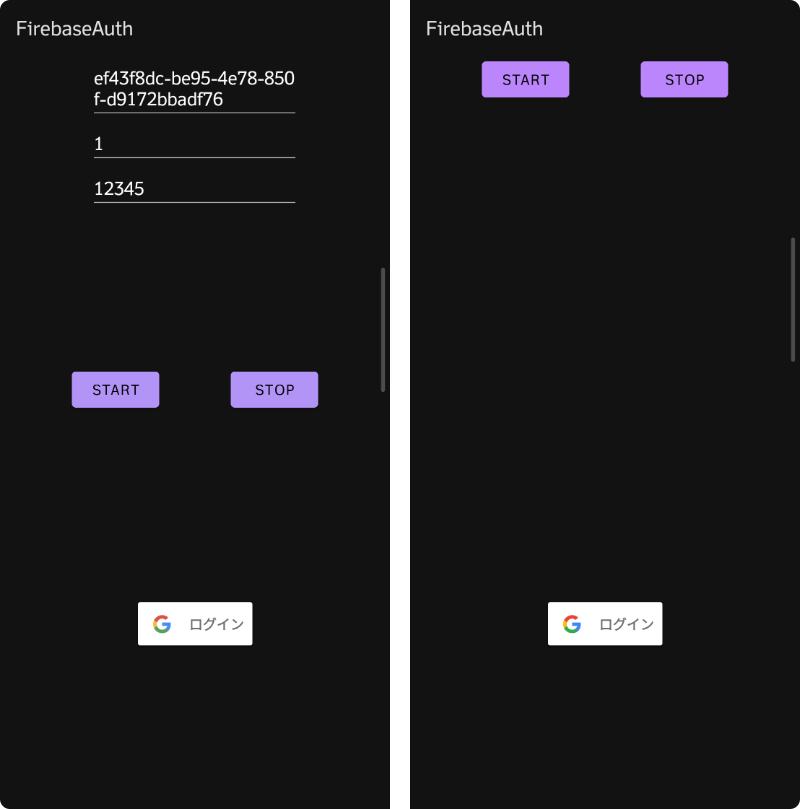
\includegraphics[width=9cm]{image/AppBeforeAfter.png}
   \caption{ユーザ向けアプリケーションにおける操作の簡略化}
   \label{multipleBPM}
 \end{figure}
また図  X   研究初期はユーザから利用しているUUID,major,minorを編集できる仕様にしていたが,複雑な操作がユーザの利便性の向上につながらないと考え取り消した.

\subsection*{4.3.2 スマホビーコンと実デバイスによるビーコンのハイブリッド活用}
スマホビーコンのみを利用する場合,様々な状況下でメンバの継続した利用が困難であるため,実デバイスによるビーコンと併用できるシステムとした.


% レジュメの内容にシチュエーションを加える 例 一時的な来訪者


\begin{table}[tbh]
  \centering
  \caption{各ビーコンのみとハイブリッド対応時の比較}
  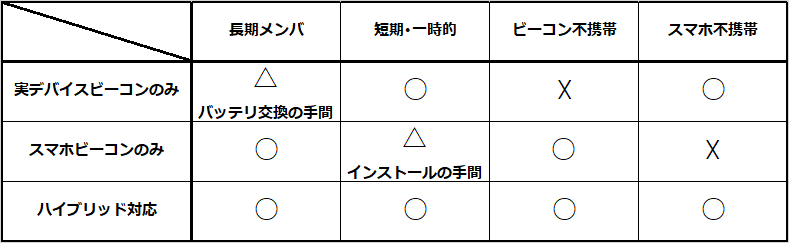
\includegraphics[width=9cm]{image/table.png}
  \label{multipleBPM}
\end{table}